\newpage
\section{velo}

\begin{figure}[h]
    \centering
    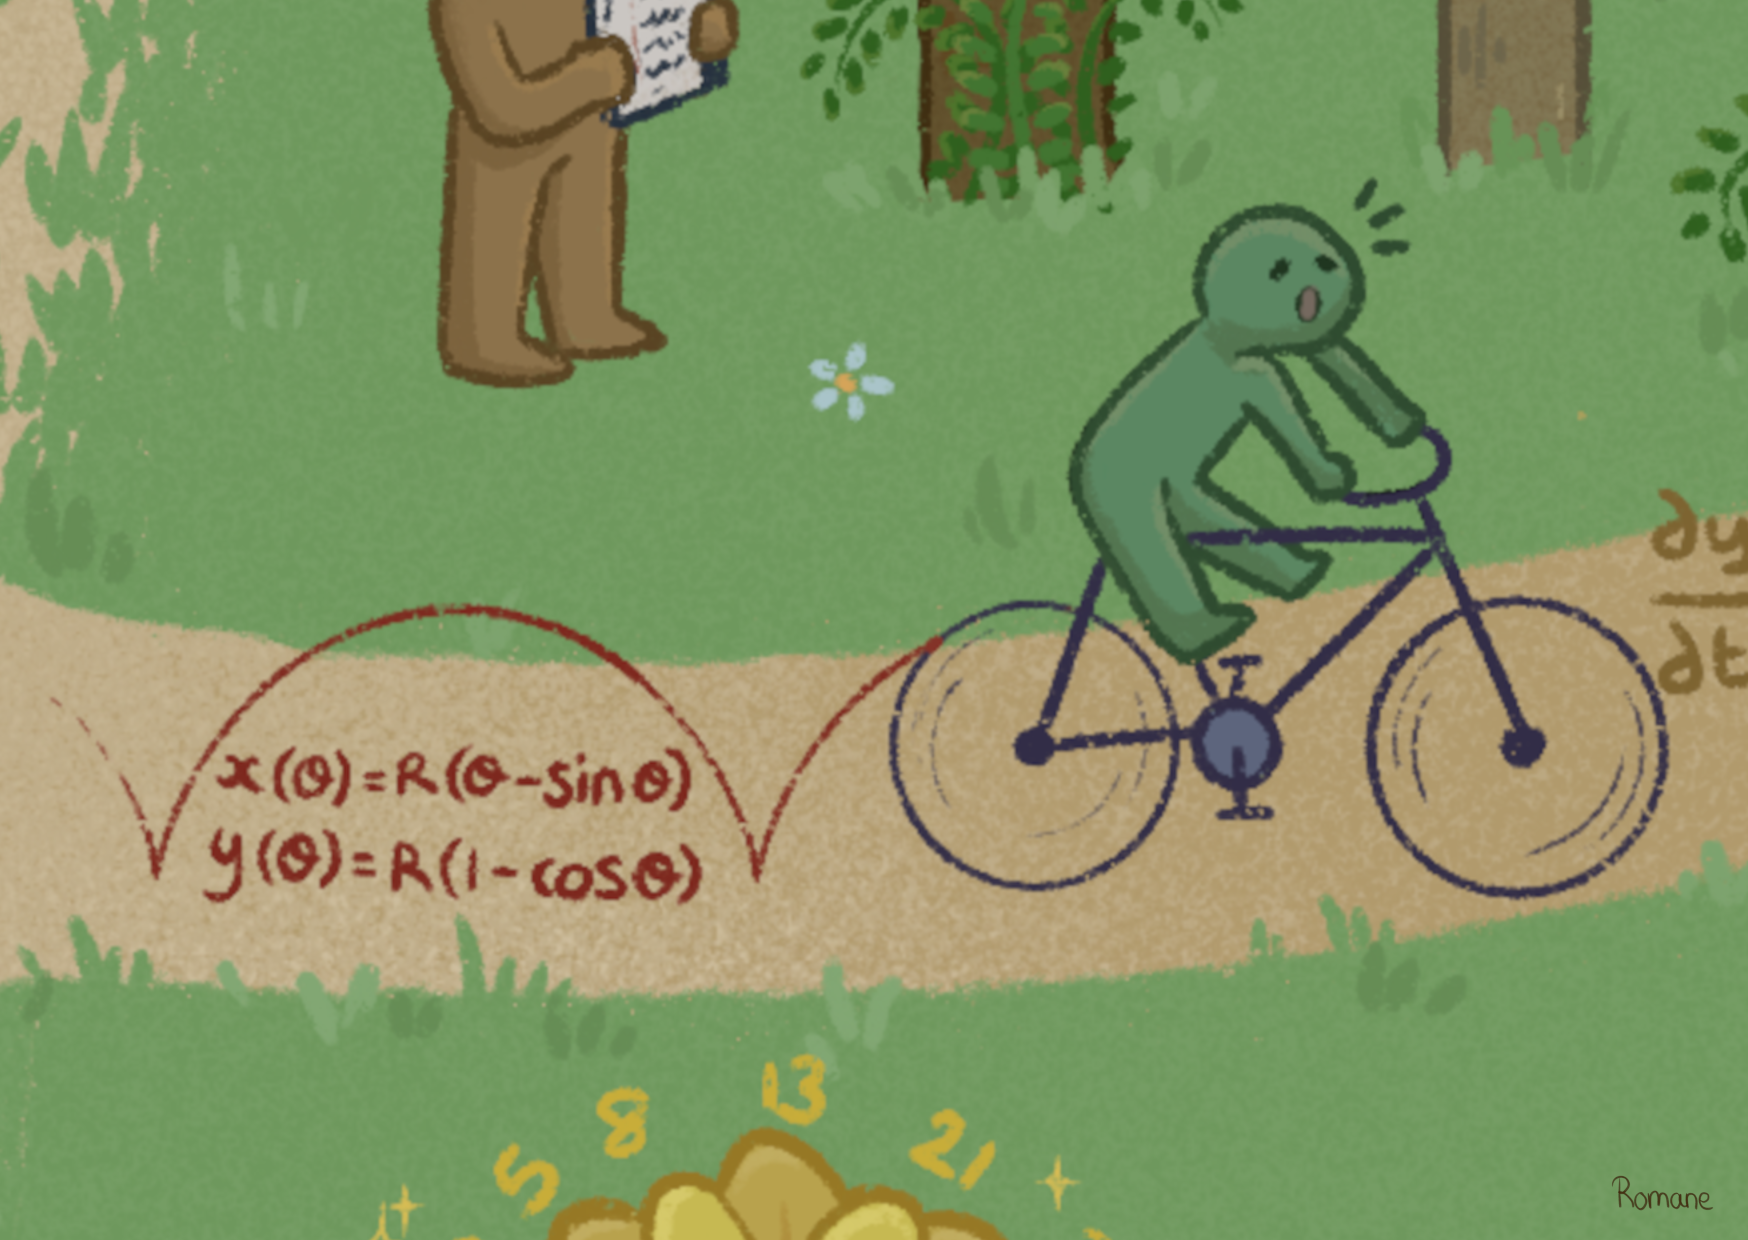
\includegraphics[height=0.5\textheight]{Cartes_postales/carte05-velo.png}\label{fig:c05}
    \caption{Carte postale: Velo}
\end{figure}

Le mouvement d'un point sur une roue de vélo est bien plus complexe qu'il n'y paraît. C'est la combinaison de deux mouvements simples, une translation et une rotation. Cela crée une courbe qu'on appelle une cycloïde, qui a des propriétés étonnantes.

\begin{figure}[h]
    \centering
    \includegraphics[height=0.1\textheight]{Images/cycloide.png}\label{fig:c05_cycloide}
    \caption{Illustration d'une cycloide inversée}
\end{figure}

Tout d'abord, en retournant cette courbe, c'est le chemin le plus rapide pour une bille de se déplacer d'un point A en hauteur à un point B plus bas. Puis, peut importe la position de départ de la bille sur cette courbe, la bille mettra toujours le même temps pour arriver tout en bas. Cette dernière propriété paraît très contre-intuitive, et pourtant ça marche super bien. L'étude de cette courbe a ouvert un champs entier en mathématiques appelé le calcul variationnel, sur lequel il y a beaucoup de recherches en cours. Voici comment on la définit:

\begin{equation*}
    \begin{cases} 
    x(\theta) = R(\theta - \sin \theta) \\
    y(\theta) = R(1 - \cos \theta) 
    \end{cases}
\end{equation*}